% Options for packages loaded elsewhere
\PassOptionsToPackage{unicode}{hyperref}
\PassOptionsToPackage{hyphens}{url}
%
\documentclass[
]{article}
\usepackage{amsmath,amssymb}
\usepackage{lmodern}
\usepackage{iftex}
\ifPDFTeX
  \usepackage[T1]{fontenc}
  \usepackage[utf8]{inputenc}
  \usepackage{textcomp} % provide euro and other symbols
\else % if luatex or xetex
  \usepackage{unicode-math}
  \defaultfontfeatures{Scale=MatchLowercase}
  \defaultfontfeatures[\rmfamily]{Ligatures=TeX,Scale=1}
\fi
% Use upquote if available, for straight quotes in verbatim environments
\IfFileExists{upquote.sty}{\usepackage{upquote}}{}
\IfFileExists{microtype.sty}{% use microtype if available
  \usepackage[]{microtype}
  \UseMicrotypeSet[protrusion]{basicmath} % disable protrusion for tt fonts
}{}
\makeatletter
\@ifundefined{KOMAClassName}{% if non-KOMA class
  \IfFileExists{parskip.sty}{%
    \usepackage{parskip}
  }{% else
    \setlength{\parindent}{0pt}
    \setlength{\parskip}{6pt plus 2pt minus 1pt}}
}{% if KOMA class
  \KOMAoptions{parskip=half}}
\makeatother
\usepackage{xcolor}
\IfFileExists{xurl.sty}{\usepackage{xurl}}{} % add URL line breaks if available
\IfFileExists{bookmark.sty}{\usepackage{bookmark}}{\usepackage{hyperref}}
\hypersetup{
  hidelinks,
  pdfcreator={LaTeX via pandoc}}
\urlstyle{same} % disable monospaced font for URLs
\usepackage[margin=1in]{geometry}
\usepackage{color}
\usepackage{fancyvrb}
\newcommand{\VerbBar}{|}
\newcommand{\VERB}{\Verb[commandchars=\\\{\}]}
\DefineVerbatimEnvironment{Highlighting}{Verbatim}{commandchars=\\\{\}}
% Add ',fontsize=\small' for more characters per line
\usepackage{framed}
\definecolor{shadecolor}{RGB}{248,248,248}
\newenvironment{Shaded}{\begin{snugshade}}{\end{snugshade}}
\newcommand{\AlertTok}[1]{\textcolor[rgb]{0.94,0.16,0.16}{#1}}
\newcommand{\AnnotationTok}[1]{\textcolor[rgb]{0.56,0.35,0.01}{\textbf{\textit{#1}}}}
\newcommand{\AttributeTok}[1]{\textcolor[rgb]{0.77,0.63,0.00}{#1}}
\newcommand{\BaseNTok}[1]{\textcolor[rgb]{0.00,0.00,0.81}{#1}}
\newcommand{\BuiltInTok}[1]{#1}
\newcommand{\CharTok}[1]{\textcolor[rgb]{0.31,0.60,0.02}{#1}}
\newcommand{\CommentTok}[1]{\textcolor[rgb]{0.56,0.35,0.01}{\textit{#1}}}
\newcommand{\CommentVarTok}[1]{\textcolor[rgb]{0.56,0.35,0.01}{\textbf{\textit{#1}}}}
\newcommand{\ConstantTok}[1]{\textcolor[rgb]{0.00,0.00,0.00}{#1}}
\newcommand{\ControlFlowTok}[1]{\textcolor[rgb]{0.13,0.29,0.53}{\textbf{#1}}}
\newcommand{\DataTypeTok}[1]{\textcolor[rgb]{0.13,0.29,0.53}{#1}}
\newcommand{\DecValTok}[1]{\textcolor[rgb]{0.00,0.00,0.81}{#1}}
\newcommand{\DocumentationTok}[1]{\textcolor[rgb]{0.56,0.35,0.01}{\textbf{\textit{#1}}}}
\newcommand{\ErrorTok}[1]{\textcolor[rgb]{0.64,0.00,0.00}{\textbf{#1}}}
\newcommand{\ExtensionTok}[1]{#1}
\newcommand{\FloatTok}[1]{\textcolor[rgb]{0.00,0.00,0.81}{#1}}
\newcommand{\FunctionTok}[1]{\textcolor[rgb]{0.00,0.00,0.00}{#1}}
\newcommand{\ImportTok}[1]{#1}
\newcommand{\InformationTok}[1]{\textcolor[rgb]{0.56,0.35,0.01}{\textbf{\textit{#1}}}}
\newcommand{\KeywordTok}[1]{\textcolor[rgb]{0.13,0.29,0.53}{\textbf{#1}}}
\newcommand{\NormalTok}[1]{#1}
\newcommand{\OperatorTok}[1]{\textcolor[rgb]{0.81,0.36,0.00}{\textbf{#1}}}
\newcommand{\OtherTok}[1]{\textcolor[rgb]{0.56,0.35,0.01}{#1}}
\newcommand{\PreprocessorTok}[1]{\textcolor[rgb]{0.56,0.35,0.01}{\textit{#1}}}
\newcommand{\RegionMarkerTok}[1]{#1}
\newcommand{\SpecialCharTok}[1]{\textcolor[rgb]{0.00,0.00,0.00}{#1}}
\newcommand{\SpecialStringTok}[1]{\textcolor[rgb]{0.31,0.60,0.02}{#1}}
\newcommand{\StringTok}[1]{\textcolor[rgb]{0.31,0.60,0.02}{#1}}
\newcommand{\VariableTok}[1]{\textcolor[rgb]{0.00,0.00,0.00}{#1}}
\newcommand{\VerbatimStringTok}[1]{\textcolor[rgb]{0.31,0.60,0.02}{#1}}
\newcommand{\WarningTok}[1]{\textcolor[rgb]{0.56,0.35,0.01}{\textbf{\textit{#1}}}}
\usepackage{graphicx}
\makeatletter
\def\maxwidth{\ifdim\Gin@nat@width>\linewidth\linewidth\else\Gin@nat@width\fi}
\def\maxheight{\ifdim\Gin@nat@height>\textheight\textheight\else\Gin@nat@height\fi}
\makeatother
% Scale images if necessary, so that they will not overflow the page
% margins by default, and it is still possible to overwrite the defaults
% using explicit options in \includegraphics[width, height, ...]{}
\setkeys{Gin}{width=\maxwidth,height=\maxheight,keepaspectratio}
% Set default figure placement to htbp
\makeatletter
\def\fps@figure{htbp}
\makeatother
\setlength{\emergencystretch}{3em} % prevent overfull lines
\providecommand{\tightlist}{%
  \setlength{\itemsep}{0pt}\setlength{\parskip}{0pt}}
\setcounter{secnumdepth}{-\maxdimen} % remove section numbering
\ifLuaTeX
  \usepackage{selnolig}  % disable illegal ligatures
\fi

\author{}
\date{\vspace{-2.5em}}

\begin{document}

\hypertarget{procesamiento-de-datos-en-tiempo-real-con-kafka}{%
\section{Procesamiento de datos en tiempo real con
kafka}\label{procesamiento-de-datos-en-tiempo-real-con-kafka}}

\textbf{Autora}: Ivonne Yanez Mendoza \textbf{Email}:
\href{mailto:ivonne@imendoza.io}{\nolinkurl{ivonne@imendoza.io}}
\textbf{GitHub}: \url{https://github.com/TiaIvonne}

\includegraphics{https://img.shields.io/badge/license-All\%20Rights\%20Reserved-red.svg}
\includegraphics{https://img.shields.io/badge/Apache\%20Kafka-7.8.0-black}
\includegraphics{https://img.shields.io/badge/status-running-green}

\hypertarget{tabla-de-contenidos}{%
\subsection{Tabla de Contenidos}\label{tabla-de-contenidos}}

\begin{enumerate}
\def\labelenumi{\arabic{enumi}.}
\tightlist
\item
  \protect\hyperlink{descripciuxf3n}{Descripción}
\item
  \protect\hyperlink{estructura-del-directorio}{Estructura del
  Directorio}
\item
  \protect\hyperlink{desarrollo-del-proyecto}{Desarrollo del Proyecto}
\item
  \protect\hyperlink{soporte}{Soporte}
\item
  \protect\hyperlink{licencia}{Licencia}
\end{enumerate}

\hypertarget{descripciuxf3n}{%
\subsection{Descripción}\label{descripciuxf3n}}

Este proyecto corresponde al modulo de Kafka y Procesamiento de datos en
tiempo real del Master en Ingenieria de datos de la Universidad
Complutense de Madrid.

Se debe construir una solución basada en Apache Kafka que permita:

\begin{enumerate}
\def\labelenumi{\arabic{enumi}.}
\item
  Procesar los datos de sensores agrícolas en tiempo real para detectar
  condiciones anormales (picos de temperatura \& humedad)
\item
  Integrar los datos de transacciones de ventas provenientes de una base
  de datos relacional MySql utilizando Kafka Connect.
\item
  Transformar los datos mediante procesamiento streaming para generar
  insights del tipo: alertas de anomalías en los sensores y ventas por
  categoría de producto cada minuto.
\end{enumerate}

\hypertarget{estructura-del-directorio}{%
\subsection{Estructura del directorio}\label{estructura-del-directorio}}

\begin{verbatim}
 0.tarea/
  ├── assets/
  ├── connectors/
  ├── datagen/
  ├── sql/
  ├── src/
  ├── pom.xml
  ├── setup.sh
  ├── shutdown.sh
  └── start_connectors.sh
\end{verbatim}

Los directorios mas relevantes para esta practica son:

\textbf{connectors}: Contienen los conectores generados en formato JSON
los cuales son necesarios para generar datos sintéticos, integrarlos con
MySql, procesar los datos en tiempo real de los sensores e integrar con
una base de datos no SQL.\\
\textbf{datagen}: Contienen la definicion del esquema y del tipo de dato
a utilizar en los connectores.\\
\textbf{sql}: Contiene la definicion de la tabla sales\_transaccions que
debe ser procesada en MySql\\
\textbf{src}: La fuente del proyecto y donde se encuentra el codigo base
para procesar los datos en tiempo real de farmaia.

Fuera de la estructura del directorio se encuentran tres scripts que se
deben ejecutar en la shell que realizan las siguientes acciones:\\
\textbf{setup.sh:} Contiene todo lo necesario para levantar Docker y
evitar tener que configurar el archivo yml en el directorio.\\
\textbf{shutdown.sh:} Para detener entorno.\\
\textbf{start\_connectors.sh:} Lanza los connectores en lote en vez de
ejecutar cada comando por separado.

\hypertarget{desarrollo-del-proyecto}{%
\subsection{Desarrollo del proyecto}\label{desarrollo-del-proyecto}}

\hypertarget{crear-los-topics}{%
\subsubsection{Crear los topics}\label{crear-los-topics}}

Se pide la creación de los siguientes topics (contenedor de mensajes)

\begin{enumerate}
\def\labelenumi{\arabic{enumi}.}
\item
  sensor-telemetry: Contiene datos de los sensores agrícolas.
\item
  sales-transactions: Contiene datos de transacciones de ventas.
\item
  sensor-alerts: Contiene alertas generadas (picos de temperatura y
  humedad) generadas al procesar los mensajes.
\item
  sales-summary: Contiene el resumen de ventas (con agregaciones)
  generadas al procesar los datos.
\end{enumerate}

Para crear los conectores es necesario comenzar lanzando el script
setup.sh que es el encargado de crear el entorno basado en docker el
cual construirá el entorno de trabajo para esta practica:

\begin{Shaded}
\begin{Highlighting}[]
 \ExtensionTok{0.tarea}\NormalTok{ git:}\ErrorTok{(}\ExtensionTok{master}\KeywordTok{)} \ExtensionTok{✗}\NormalTok{ ./setup.sh}
  \ExtensionTok{✔}\NormalTok{ Container connect  Started 5.6s }
\ExtensionTok{Esperando}\NormalTok{ reinicio contenedor connect}
\ExtensionTok{OK}
\end{Highlighting}
\end{Shaded}

\begin{figure}
\centering
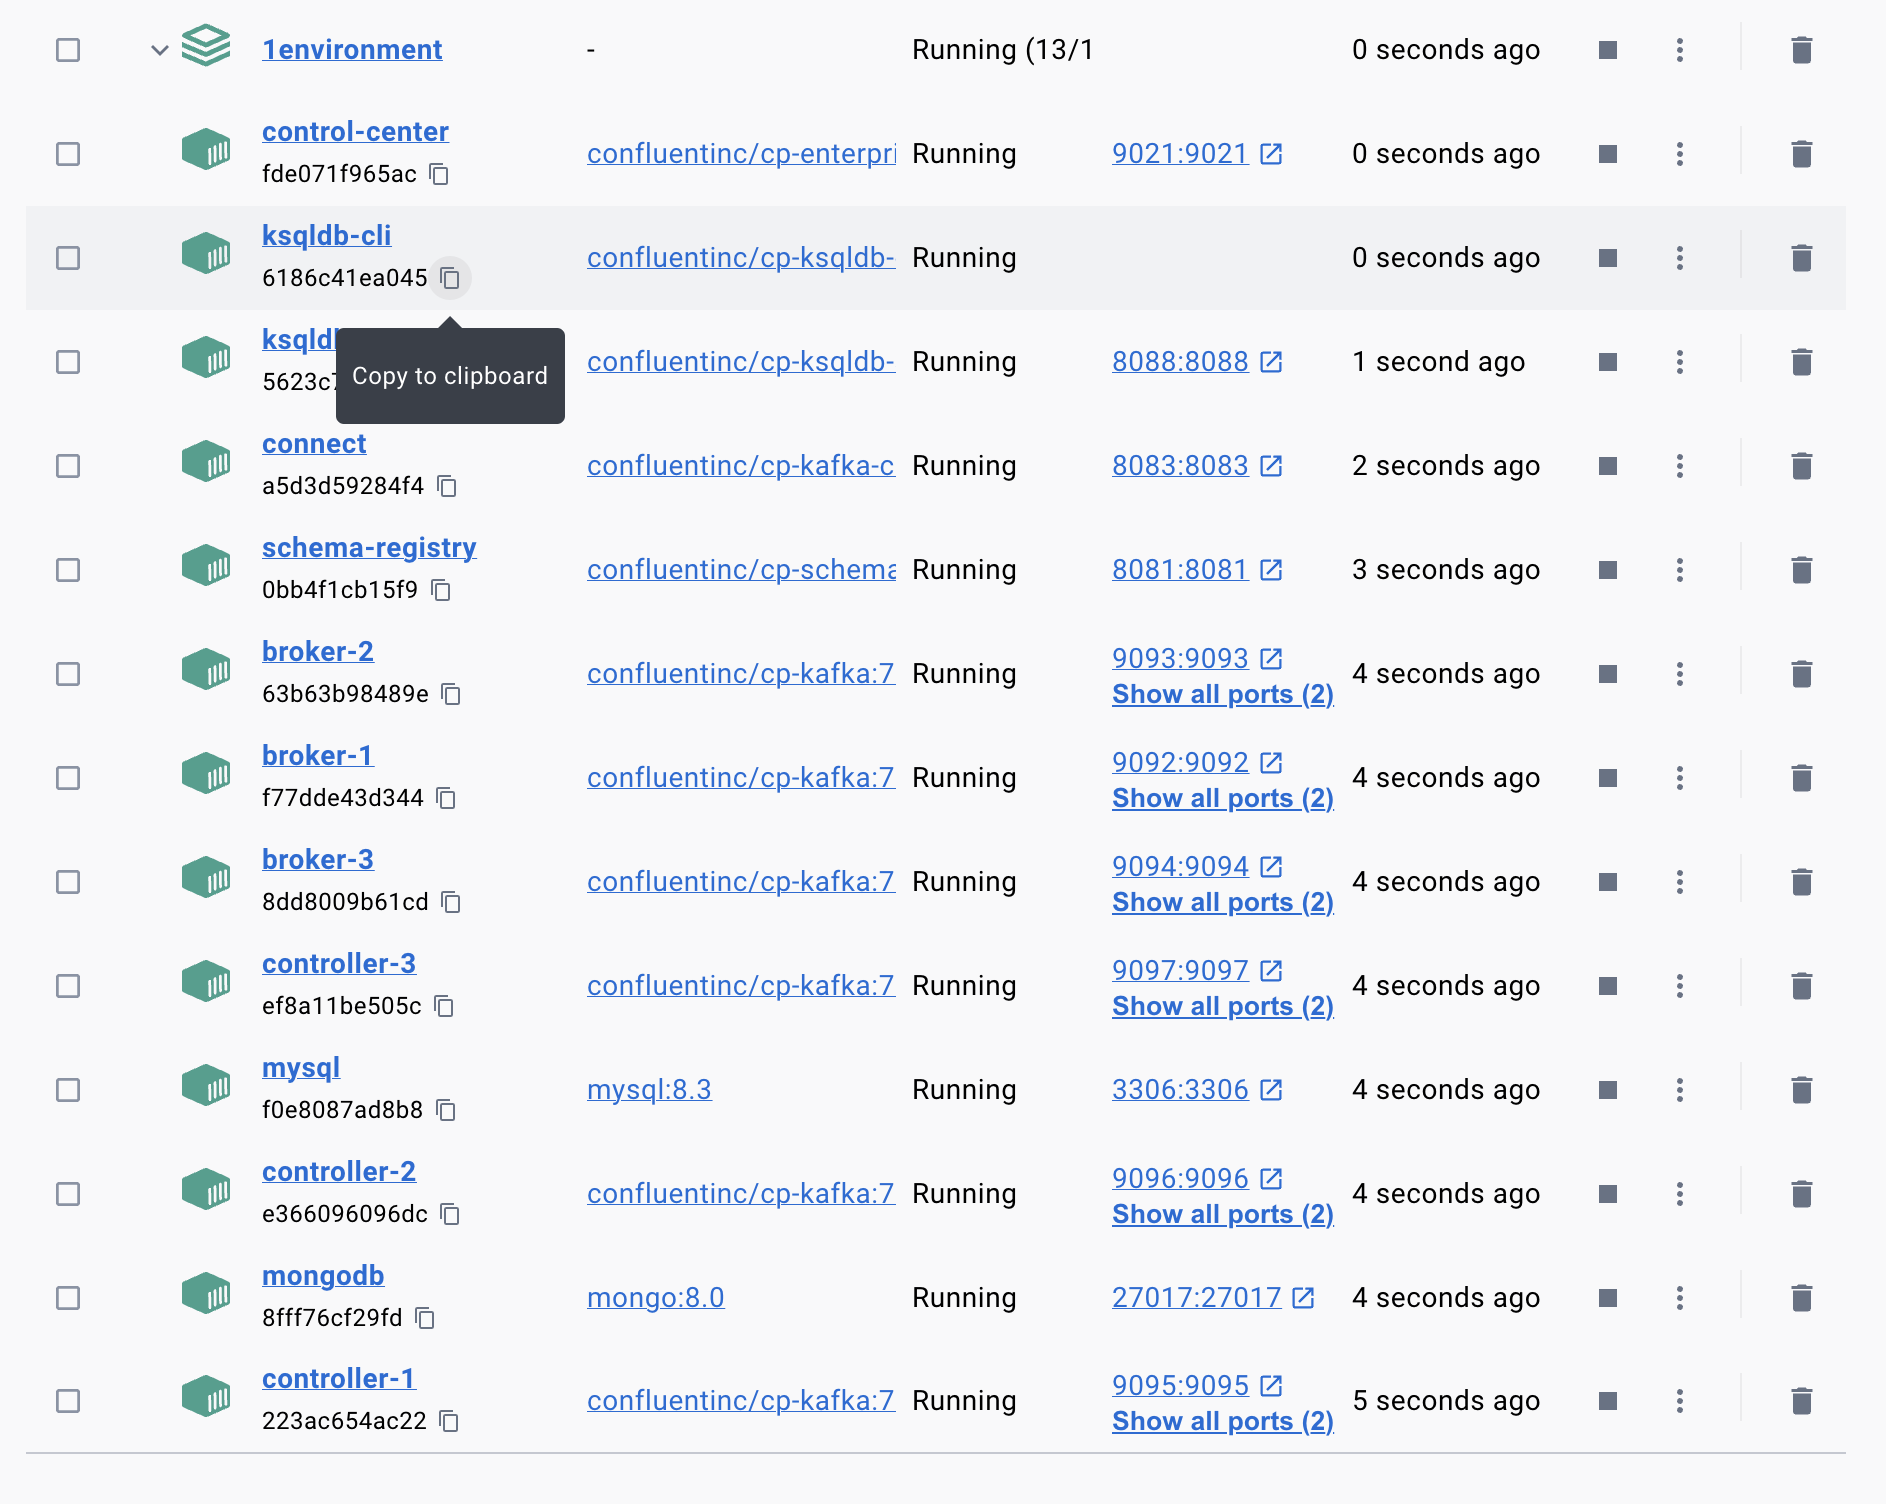
\includegraphics{assets/docker-running.png}
\caption{Docker Running}
\end{figure}

Una vez que esta corriendo docker es momento de entrar en la consola
interactiva y crear los topics

\begin{Shaded}
\begin{Highlighting}[]
\NormalTok{0.tarea git:(master) ✗ docker exec {-}it broker{-}1 /bin/bash}
\end{Highlighting}
\end{Shaded}

Una vez en la consola se lanzan los siguientes comandos para crear los
topicos:

\begin{Shaded}
\begin{Highlighting}[]
\ExtensionTok{[appuser@broker{-}1}\NormalTok{ \textasciitilde{}]$ kafka{-}topics }\AttributeTok{{-}{-}bootstrap{-}server}\NormalTok{ broker{-}1:29092 }\AttributeTok{{-}{-}create} \AttributeTok{{-}{-}topic}\NormalTok{ sensor{-}telemetry }\AttributeTok{{-}{-}partitions}\NormalTok{ 4 }\AttributeTok{{-}{-}replication{-}factor}\NormalTok{ 2 }\AttributeTok{{-}{-}config}\NormalTok{ max.message.bytes=64000 }\AttributeTok{{-}{-}config}\NormalTok{ flush.messages=1}
\end{Highlighting}
\end{Shaded}

Nota personal: Esto puede ser un poco tedioso por cada topic, por lo que
he creado un script de bash que hace esta tarea por cada topic a
crear.\\
El script se encuentra en el directorio raiz con el nombre de
\textbf{create-topics.sh}.

\begin{Shaded}
\begin{Highlighting}[]
\VariableTok{BOOTSTRAP\_SERVER}\OperatorTok{=}\StringTok{"broker{-}1:29092"}
  \VariableTok{PARTITIONS}\OperatorTok{=}\NormalTok{4}
  \VariableTok{REPLICATION\_FACTOR}\OperatorTok{=}\NormalTok{2}

\VariableTok{TOPICS}\OperatorTok{=}\VariableTok{(}
      \StringTok{"sensor{-}telemetry"}
      \StringTok{"sales{-}transactions"}
      \StringTok{"sensor{-}alerts"}
      \StringTok{"sales{-}summary"}
\VariableTok{)}

\ControlFlowTok{for}\NormalTok{ TOPIC }\KeywordTok{in} \StringTok{"}\VariableTok{$\{TOPICS}\OperatorTok{[@]}\VariableTok{\}}\StringTok{"}\KeywordTok{;} \ControlFlowTok{do}
    \BuiltInTok{echo} \StringTok{"Creando topic: }\VariableTok{$TOPIC}\StringTok{"}
    \ExtensionTok{docker}\NormalTok{ exec broker{-}1 kafka{-}topics }\DataTypeTok{\textbackslash{}}
        \AttributeTok{{-}{-}bootstrap{-}server} \VariableTok{$BOOTSTRAP\_SERVER} \DataTypeTok{\textbackslash{}}
        \AttributeTok{{-}{-}create} \DataTypeTok{\textbackslash{}}
        \AttributeTok{{-}{-}topic} \VariableTok{$TOPIC} \DataTypeTok{\textbackslash{}}
        \AttributeTok{{-}{-}partitions} \VariableTok{$PARTITIONS} \DataTypeTok{\textbackslash{}}
        \AttributeTok{{-}{-}replication{-}factor} \VariableTok{$REPLICATION\_FACTOR} \DataTypeTok{\textbackslash{}}
        \AttributeTok{{-}{-}config}\NormalTok{ max.message.bytes=64000 }\DataTypeTok{\textbackslash{}}
        \AttributeTok{{-}{-}config}\NormalTok{ flush.messages=1}
    \ControlFlowTok{done}
\end{Highlighting}
\end{Shaded}

Por consola se pueden ver los topics creados

\begin{Shaded}
\begin{Highlighting}[]
\ExtensionTok{kafka{-}topics} \AttributeTok{{-}{-}bootstrap{-}server}\NormalTok{ broker{-}1:29092 }\AttributeTok{{-}{-}list}
\end{Highlighting}
\end{Shaded}

O en el control center:

\begin{figure}
\centering
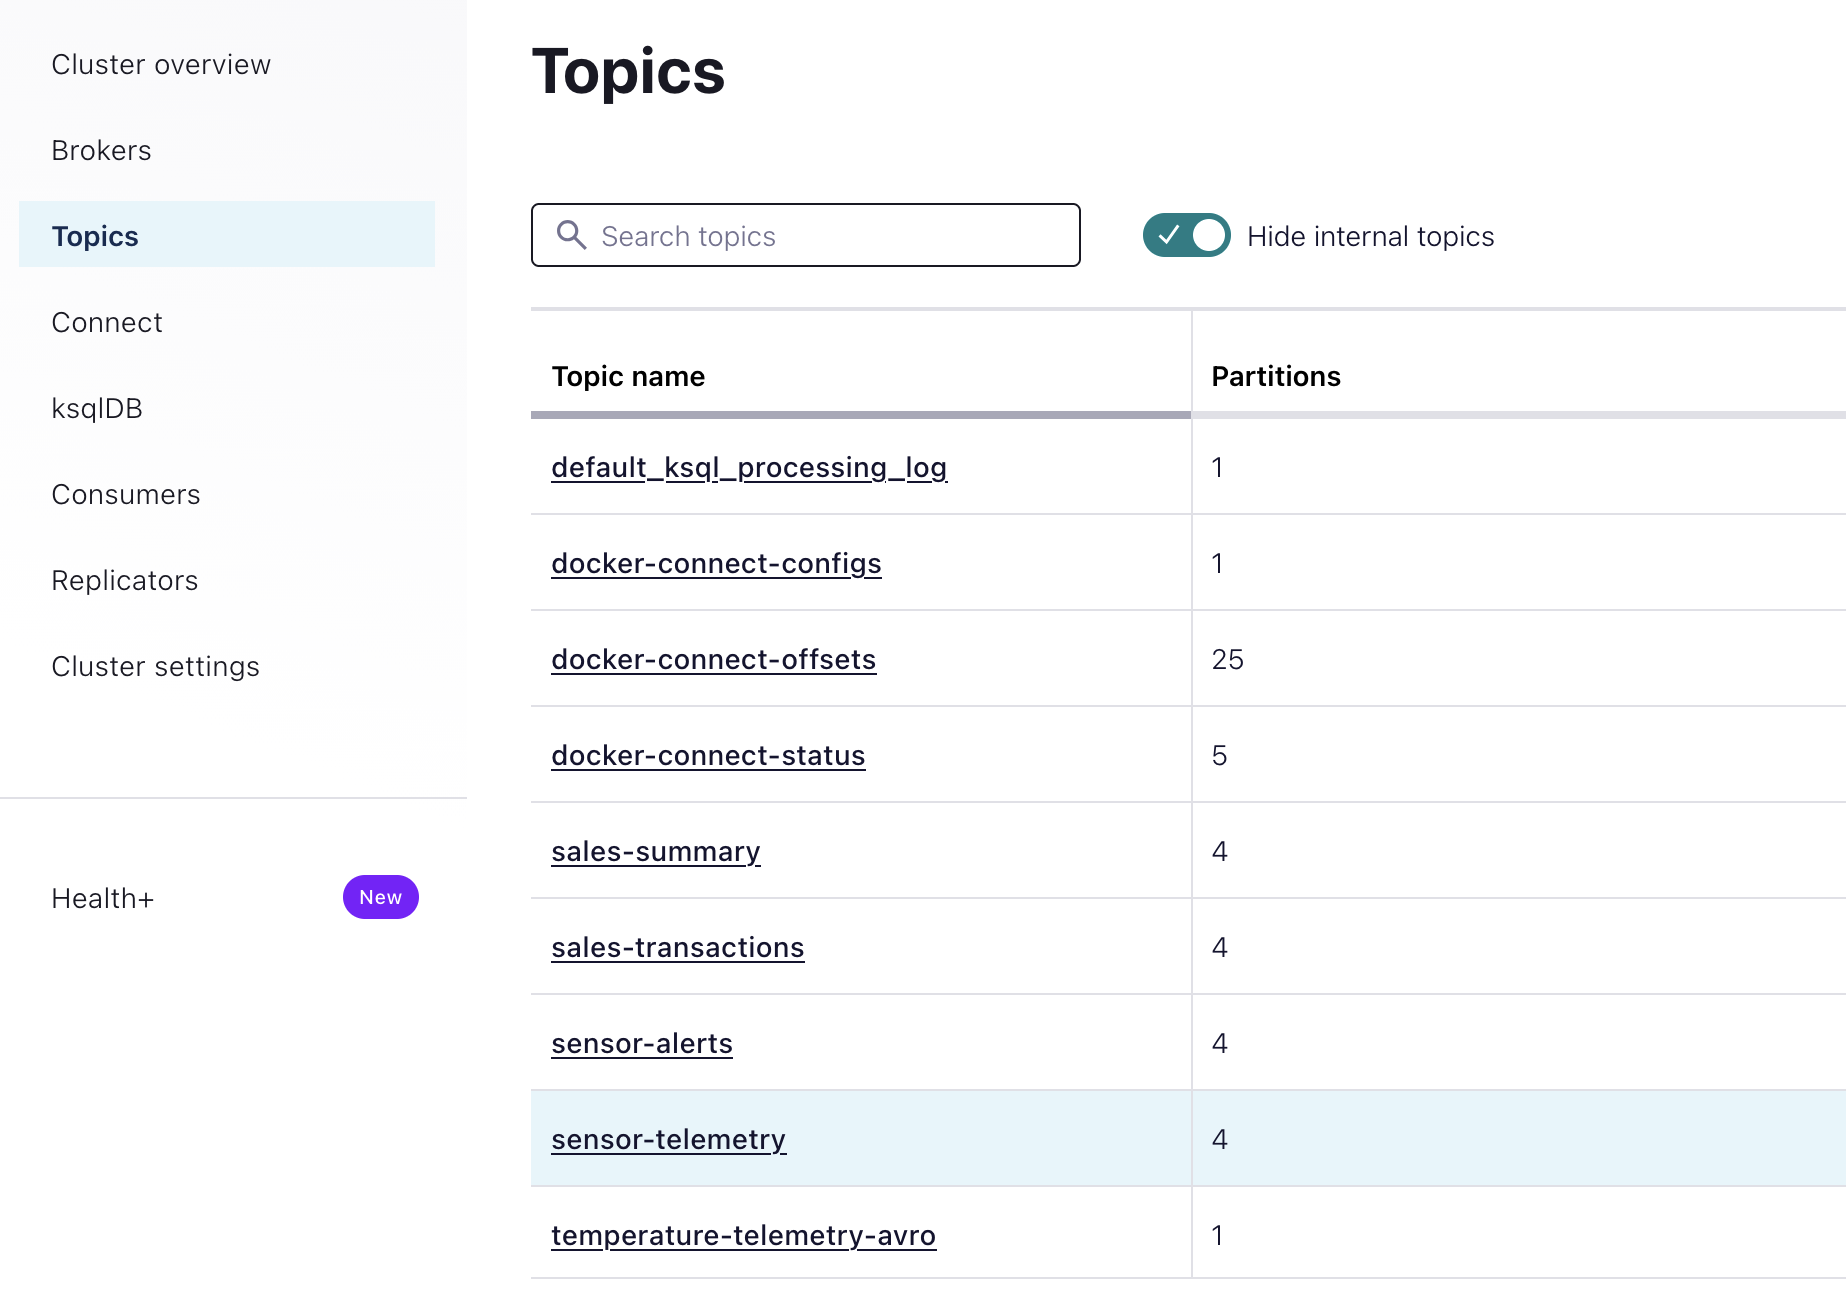
\includegraphics{assets/crear-topics.png}
\caption{Control Center}
\end{figure}

\hypertarget{licencia}{%
\subsection{Licencia}\label{licencia}}

Todos los derechos reservados

\end{document}
